\documentclass[PI,LAB]{HSEUniversity}

\usepackage{graphicx}
\graphicspath{ {img/} }

\usepackage{hyperref}
\hypersetup{
    colorlinks=true,
    linkcolor=black,
    filecolor=magenta,      
    urlcolor=cyan,
}

\title{Организация паттернов проектирования. Поведенческий паттерн <<Интерпретатор>>}
\author{Рязанов Иван Дмитриевич}
\supervisor{к.т.н., доцент кафедры Информационных технологий в бизнесе НИУ ВШЭ-Пермь}{А.В.~Кычкин}
\Year{2020}

\begin{document}
\maketitle
\chapter{Паттерн <<Интерпретатор>>}
\textbf{Название и классификация паттерна.}
Интерпретатор — паттерн, определяющий представление грамматики для заданного языка и интерпретатор предложений этого языка. Как правило, данный шаблон проектирования применяется для часто повторяющихся операций.

\textbf{Назначение.}
Паттерн <<Интерпретатор>> определяет грамматику простого языка для проблемной области, представляет грамматические правила в виде языковых предложений и интерпретирует их для решения задачи. Для представления каждого грамматического правила паттерн <<Интерпретатор>> использует отдельный класс. А так как грамматика, как правило, имеет иерархическую структуру, то иерархия наследования классов хорошо подходит для ее описания.

\begin{enumerate}
	\item Для заданного языка определяет представление его грамматики, а также интерпретатор предложений этого языка.
	\item Отображает проблемную область в язык, язык – в грамматику, а грамматику – в иерархии объектно-ориентированного проектирования.
\end{enumerate}

\textbf{Применимость.}
Интерпретатор следует использовать, когда необходимо интерпретировать запись в другом языке и т.д. Как один из примеров может служить перевод римских цифр в арабские. В общих случаях паттерн следует использовать тогда, когда задача соответствует следующему описанию:
- пусть в некоторой, хорошо определенной области, периодически случается некоторая проблема. Если эта область может быть описана некоторым <<языком>>, то проблема может быть легко решена с помощью <<интерпретирующей машины>>.

\clearpage

\begin{figure}[p]
  \centering
  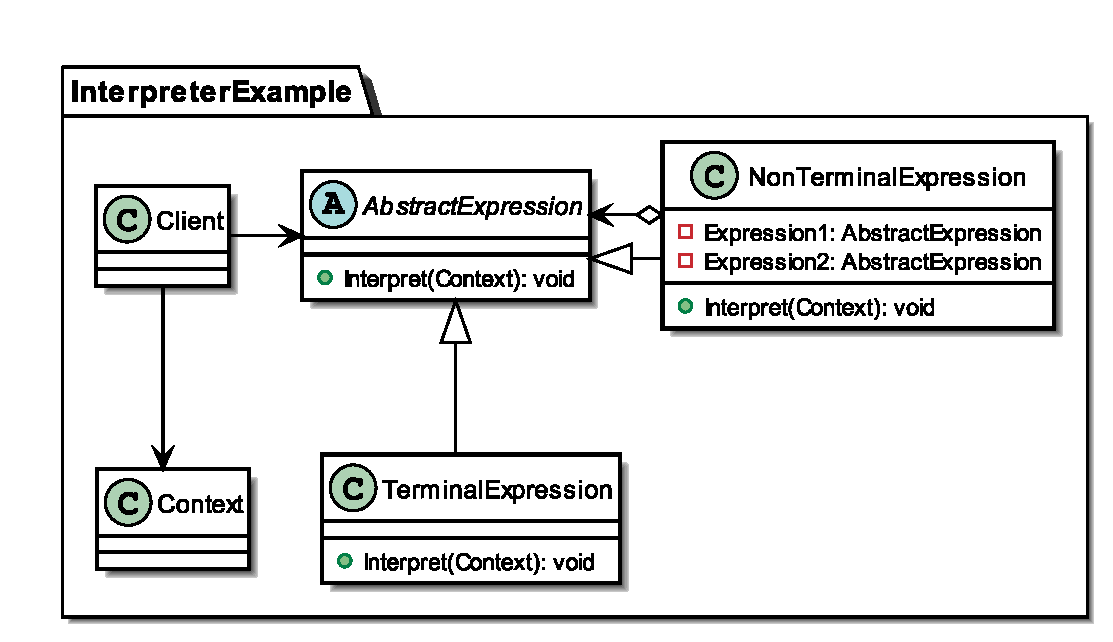
\includegraphics[scale=0.7]{Interpreter_CD.eps}
  \caption{Диаграмма классов паттерна <<Интерпретатор>>}
\end{figure}

\begin{figure}[p]
  \centering
  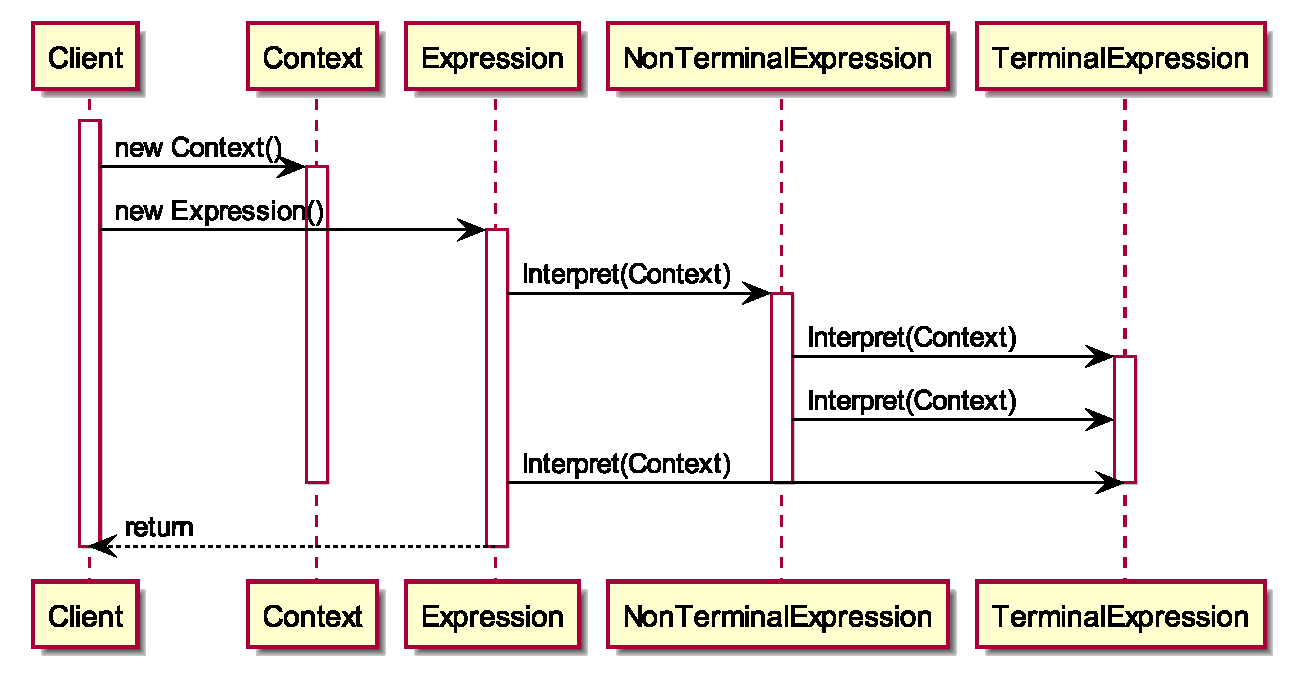
\includegraphics[scale=0.75]{Interpreter_SD.eps}
  \caption{Диаграмма последовательности паттерна <<Интерпретатор>>}
\end{figure}
\clearpage

\textbf{Участники}

\begin{enumerate}
    \item \code{AbstractExpression}: определяет интерфейс выражения, объявляет метод \code{Interpret()}.
    \item \code{TerminalExpression}: терминальное выражение, реализует метод \code{Interpret}() для терминальных символов грамматики. Для каждого символа грамматики создается свой объект TerminalExpression.
    \item \code{NonterminalExpression}: нетерминальное выражение, представляет правило грамматики. Для каждого отдельного правила грамматики создается свой объект NonterminalExpression.
    \item \code{Context}: содержит общую для интерпретатора информацию. Может использоваться объектами терминальных и нетерминальных выражений для сохранения состояния операций и последующего доступа к сохраненному состоянию.
    \item \code{Client}: строит предложения языка с данной грамматикой в виде абстрактного синтаксического дерева, узлами которого являются объекты \code{TerminalExpression} и \code{NonterminalExpression}.
\end{enumerate}

\textbf{Отношения.}

Клиент строит (или получает в готовом виде) предложение в виде абстрактного синтаксического дерева, в узлах которого находятся объекты классов \code{NonterminalExpression} и \code{TerminalExpression}. Затем клиент инициализирует контекст и вызывает операцию \code{Interpret()};
В каждом узле вида \code{NonterminalExpression} через операции \code{Interpret} определяется операция \code{Interpret} для каждого подвыражения. Для класса \code{TerminalExpression} операция \code{Interpret} определяет базу рекурсии;
Операции \code{Interpret} в каждом узле используют контекст для сохранения и доступа к состоянию интерпретатора

\textbf{Плюсы и минусы.}

Плюсы:
\begin{enumerate}
	\item Грамматику легко изменять и расширять. Поскольку для представления грамматических правил в паттерне используются классы, то для изменения - или расширения грамматики можно применять наследование. Существующие выражения можно модифицировать постепенно, а новые определять как вариации старых (компоновка, агрегация старых).
	\item Простая реализация грамматики. Реализации классов, описывающих узлы абстрактного синтаксического дерева, похожи. Такие классы легко кодировать, а зачастую их может автоматически сгенерировать компилятор или генератор синтаксических анализаторов.
\end{enumerate}

Минусы:
\begin{enumerate}
	\item Сложные грамматики трудно сопровождать. В паттерне интерпретатор определяется по меньшей мере один класс для каждого правила грамматики (для правил, определенных с помощью формы Бэкуса-Наура – BNF, может понадобиться и более одного класса). Поэтому сопровождение грамматики с большим числом правил иногда оказывается трудной задачей.
\end{enumerate}

\textbf{Области применения}

\begin{enumerate}
	\item Интерпретаторы языков программирования
	\item Интерпретация и вычисление алгебраических выражений
\end{enumerate}

\chapter{Проектирование и реализация}
\section{Проектирование}
С помощью паттерна <<Интерпретатор>> попробуем реализовать интерпретатор эзотерического языка программирования <<Brainfuck>> (\emph{вынос мозга}).
Язык состоит из 8 операторов:

\begin{enumerate}
  \item \code{>} --- переход к следующей ячейке памяти.
  \item \code{<} --- переход к предыдущей ячейке памяти.
  \item \code{+} --- увеличить значение в текущей ячейке на 1.
  \item \code{-} --- уменьшить значение в текущей ячейке на 1.
  \item \code{.} --- напечатать значение из текущей ячейки.
  \item \code{,} --- ввести извне значение и сохранить в текущей ячейке.
  \item \code{[} --- если значение текущей ячейки ноль, перейти вперёд по тексту программы на ячейку, следующую за соответствующей \code{]} (с учётом вложенности).
  \item \code{]} --- если значение текущей ячейки не нуль, перейти назад по тексту программы на символ \code{[} (с учётом вложенности).
\end{enumerate}

Операторы \code{[} и \code{]} используются для объявления цикла \code{while~(memory[pointer]~!=~0)~\{...\}}.
Всего память состоит из 30000 байт, поэтому её можно реализовать массивом \code{byte[30000]}.
Изначально во всех ячейках памяти записаны нули.

Пример программы <<Hello World>>:
\begin{verbatim}
  ++++++++[>++++[>++>+++>+++>+<<<<-]
  >+>+>->>+[<]<-]>>.>---.+++++++..+++.>>
  .<-.<.+++.------.--------.>>+.>++.
\end{verbatim}

\clearpage

 \begin{figure}[h]
   \centering
   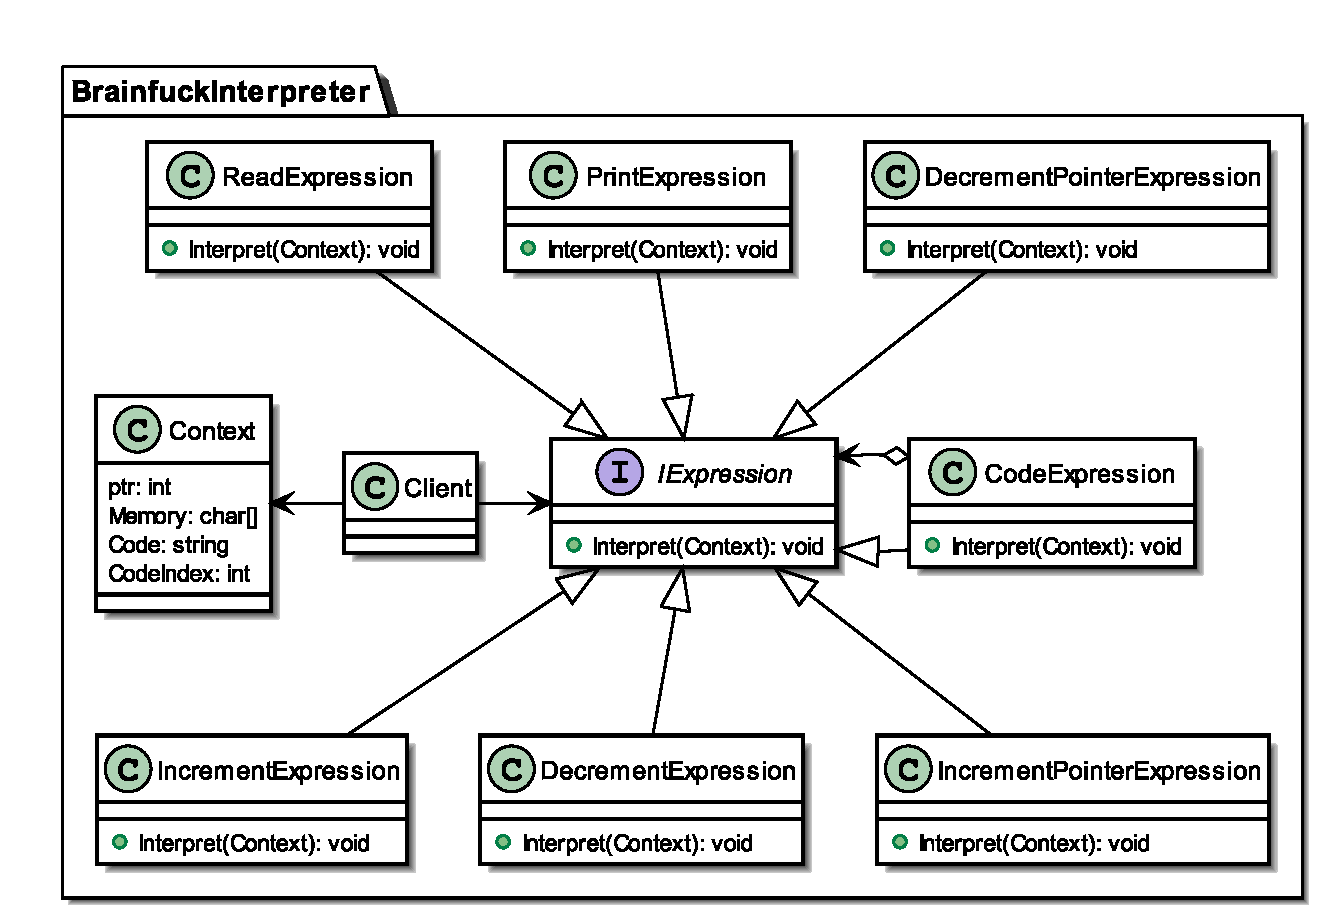
\includegraphics[scale=0.75]{Task_CD.eps}
   \caption{Диаграмма классов}
   \label{fig:Task_CD}
 \end{figure}

\textbf{Участники}

\begin{enumerate}
  \item \code{IExpression}: определяет интерфейс выражения, объявляет метод \code{Interpret()}.
  \item \code{IncrementExpression},~\code{DecrementExpression},~\code{IncrementPointerExpression}, \code{DecrementPointerExpression}, \code{PrintExpression}, \code{ReadExpression}: терминальные выражение, реализуют метод \code{Interpret}() для терминальных (\code{<>+-.,}) символов грамматики.
  \item \code{CodeExpression}: нетерминальное выражение. Используется для интерпретации кода и для выполнения циклов.
  \item \code{Context}: содержит общую для интерпретатора информацию (память, указатель на текущую ячейку, код программы, указатель на текущую инструкцию в коде).
\end{enumerate}

\section{Реализация}
Реализация паттерна <<Интерпретатор>> находится в git-репозитории по ссылке: \href{https://github.com/rovany706/design-patterns/tree/master/Interpreter/BrainfuckInterpreter}{github.com}

\end{document}
